
In this section we will analyze some of the results of our experiments and discuss their implications.

\subsection{Worker answers vs ratings}
\label{sec:analysis:answers_vs_ratings}

First, let's look at the contribution of additional answers and answer ratings provided by the workers.
These two types of contributions are complimentary to each other and attempts to solve different problems.
Table \ref{table:performance} shows the performance of our question answering system using each of these types of feedback independently.
The results demonstrate that both answers and ratings have positive effect on the performance.
Even with limited time, workers were able to reliably rate candidate answers, which helped the system to select a better final answer and improve the model precision.
However, this method doesn't help the system in cases, when it wasn't able to generate a good candidate in the first place, therefore using ratings only has lower average answer score than using worker generated answers.
By asking the crowd to provide a response if they can answer the question, CRQA covers this gap, which is important as in a real scenario even a fair answer would probably be better for the user than no answer at all.
Of course, given limited time and the fact that a random worker might not possess an expertise required to answer the question, such answers don't always perfectly answer the question.
\todo[inline]{One of the limitations of the paper is that it does not discuss the type of topics / questions on which the approach  works well and the type of topics on which the use of crowdsourcing fails.}
Table \ref{table:answer_examples} gives some examples of worker generated answers with low and high quality scores.

To summarize our answer to RQ2, ratings of answer candidates and worker generated answers both have similar positive effect on the performance of our question answering system.
What is more important, the contributions are independent and therefore it is beneficial to use both of them in the final system.

\begin{table*}[ht]
\centering
\begin{tabular}{| p{10.5cm} | p{5cm} | c |}
\hline
Question & Answer & Score \\
\hline
 Is Gotu Kola a good herb for mental health? How long does it take to work?? & yes & 1.66\\
 \hline
Can I write any number on line number 5 of a W2?  would like to set up my W2 were I get the most out of my paycheck and not have to pay taxes at the end of the year... & W2 & 1.33\\
 \hline
I need help with my mum? Something traumatic happened to me about 4 years ago i randomly asked my mother why when I lived with you in your home country a man that was our neighbour used to call me his daughter and the younger kids that lived there called me there cousins and one boy called me his sister? & yes & 1.0\\
\hline
\hline
 Is it bad not wanting to visit your family? & It's nt bad. Just be honest with them. They may be upset but they should understand & 3.0 \\
 \hline
Any health concerns with whey protein? So I workout 3-5 days a week and i drink a whey protein isolate after each workout. Since I workout almost everyday, is it ok for me to just drink a shake everyday?.. & As long as you use it as directed, there should not be any major problems.  You may want to consult your doctor just in case, but I would not be too concerned. & 3.0\\
\hline
Foot pain unable to walk? Hi so today woke with some pain, I'm able to put weight on my heel with no problem or pain.  But  the area between my heel and toes hurts really bad when I try to go with the motion of taking a step. Its not swollen and I don't remember hurting it at all & Possible gout in your foot, also possible you may have strained it during the previous day. & 3.0\\
\hline
What is a good remedy/medicine for stomach aches? Specifically ones caused by stress or anxiety? & Chamomile tea should help & 3.66\\
\hline
\end{tabular}
\caption{Examples of answers provided by the crowd workers and their average quality scores}
\label{table:answer_examples}
\end{table*}

\subsection{Selection of answer candidate for rating}
\label{sec:analysis:order}

Predicting the quality of answers and ranking them to select the best is one of the main challenges in automated question answering \cite{surdeanu2011learning}.
External feedback, such as noisy answer ratings, obtained from the crowd workers, provide valuable information, which, as our results demonstrate, can help a QA system to better re-rank the answers.
However, the capacity of crowdsourcing for answer ratings are obviously limited, as systems often are dealing with hundreds and thousands of answer candidates for a given question.
In this work, we made a choice to rate only top-7 answers according the automated system ranking.
This decision was made based on the average number of ratings workers could provide in the allotted time\footnote{The answers were posted for rating automatically after an automated system was done with candidate generation and ranking. On average users had $\sim$ 35 seconds to provide the ratings.}.
However, the order in which the answers are shown can also have a strong effect on the system performance, because the answers are typically rated one by one in the order they are displayed on the screen.
Our system included two strategies for answer ordering: random or according to their ranking score.
The former strategy provides a uniform coverage for all the answers selected for rating, while the later puts more emphasis on the currently top scoring candidates.
We randomly selected one of the strategies for each user and question.
To analyze the performance of each of the strategies we compute the average score of answers, generated using the corresponding ratings.
The average score for answers generating when candidates are shuffled is 2.508, and it's 2.539 when the candidates are sorted according to their model ranking score.
This suggests, that it's beneficial to allocate more of the workers attention on the top scoring candidate answers.

\subsection{Cost analysis}
\label{sec:analysis:cost}

The results of our experiments clearly demonstrated that crowdsourcing can improve the performance of near real-time question answering system.
The next reasonable question is what is the price of this improvement.
In our study we paid workers \$1.00 per single 15 minutes task, and each 15 minutes we had 10 assignments, which translates to \$15.00 per 15 minutes.
Overall, our experiment cost \$0.88 per question, and in this section we will discuss some ideas to reduce this cost.

First, we will study the effect of the number of workers on the performance of our CRQA system.
For this experiment we randomly sampled certain percentage of workers and removed all contributions (answers and ratings) of others.
Figure \ref{fig:nworkers_vs_quality} plots the dependency of the performance of our QA system on the number of workers.

\begin{figure*}[h!t]
  \begin{subfigure}[t]{0.5\textwidth}
	\centering
	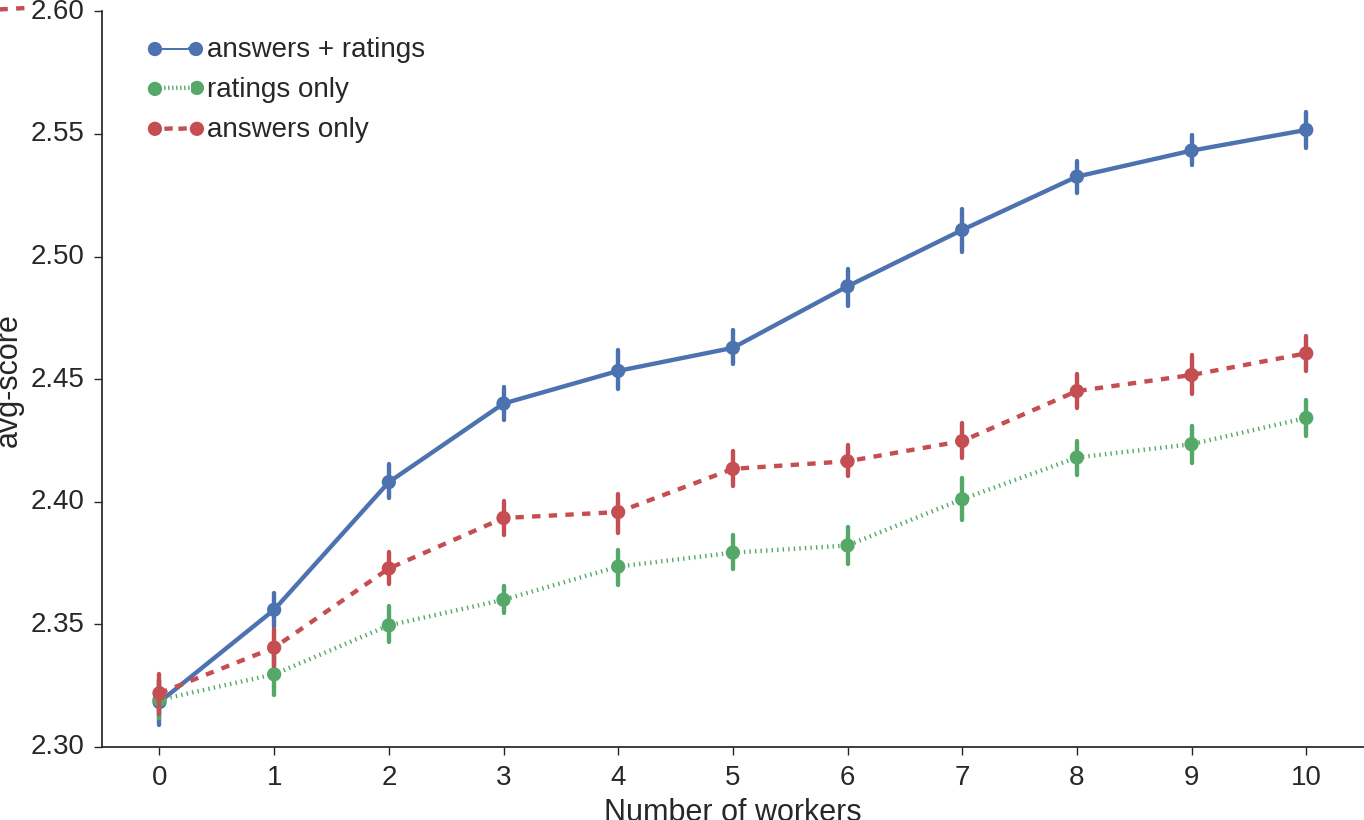
\includegraphics[width=\textwidth]{img/nworkers_vs_accuracy}
	\caption{avg-score: Average score per question}
	\label{fig:nworkers_vs_accuracy}
  \end{subfigure}
  \begin{subfigure}[t]{0.5\textwidth}
	\centering
	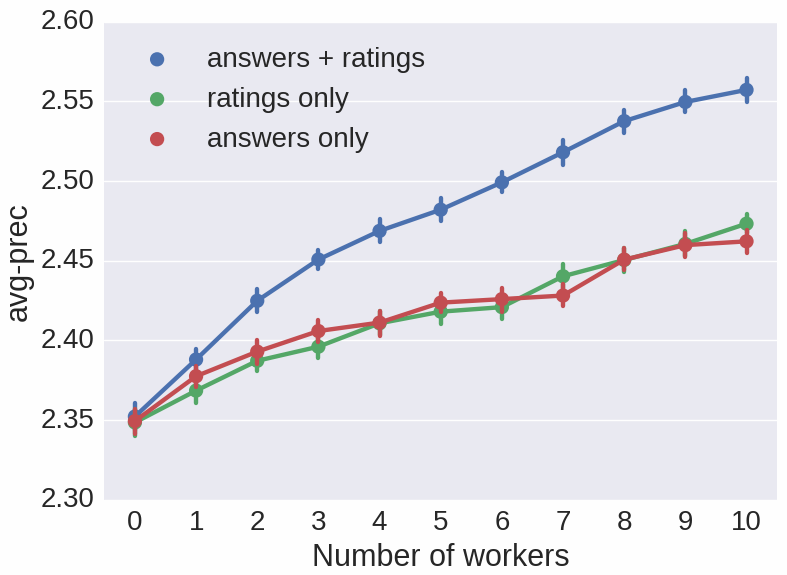
\includegraphics[width=\textwidth]{img/nworkers_vs_precision}
	\caption{avg-prec: Average score per answer (ignoring non-answered questions)}
	\label{fig:nworkers_vs_precision}
  \end{subfigure}
	\caption{Plot showing how the quality of the final answer depends on the number of workers per question}
	\label{fig:nworkers_vs_quality}
\end{figure*}

Obviously more workers mean more reliable answer ratings and more answer candidates, which improves the performance of the question answering system.
However, we can observe diminishing returns, as the cost per extra gain in performance metrics decreases as the number of workers grow.
Half of the overall performance improvement could be achieved with only 3 workers per question, which would save 70\% of the costs.

An alternative cost-reduction strategy is selective triggering of crowdsourcing, which would only ask for workers feedback for some of the questions.
Such a strategy would be necessary to scale a crowd-powered question answering system to a higher volume of questions.
There are multiple different approaches for such selective crowdsourcing: \textit{e.g.} a system can only ask for crowd contributions if it didn't generate enough candidate answers or the predicted quality of the top scoring candidates is low \cite{carmel2010estimating,he2006query}.
We leave this questions for the future work, as here we focused on the scenario, proposed by the organizers of the TREC LiveQA shared tasks, where questions arrive one by one and it's possible to utilize crowd input for every questions.

To summarize and answer RQ3, in the explored real-time QA scenario it is possible to reduce the costs of crowdsourcing by reducing the number of workers, although with some performance losses.
Our analysis suggests that paying 30\% of the original cost would give 50\% of the performance improvement.
% THE ANSWER IS KIND OF WEAK...

% \subsection{Time of day}
% Does the quality differ in different times of day?